\part{Práctica 3: Diseño del Sistema}

\section{Introducción}

Esta práctica da continuidad al proceso de modelado iniciado en la Práctica 2, donde se definieron los requisitos funcionales y no funcionales del sistema. A partir de dichos requisitos, se procede a construir los cuatro modelos arquitectónicos que propone la metodología UWE (UML-based Web Engineering): Modelo de Contenido, Modelo de Navegación, Modelo de Proceso y Modelo de Presentación.

Cada modelo responde a una dimensión distinta del sistema y, en conjunto, garantizan la trazabilidad desde los requisitos capturados hasta la implementación final. Tal como lo establece Koch et al. \cite{UWE2014}, el diseño debe partir siempre de los requisitos validados y progresar de lo general (estructura de datos) a lo particular (interfaz de usuario).

\section{Modelo de Contenido}

\subsection{Objetivo}
El Modelo de Contenido representa la estructura estática del sistema: las entidades (clases) que almacenan información y las relaciones entre ellas. Responde a la pregunta: ¿Qué datos maneja el sistema y cómo se relacionan entre sí?

\subsection{Diagrama de Clases}

\begin{figure}[H]
    \centering
    \resizebox{\textwidth}{!}{%
    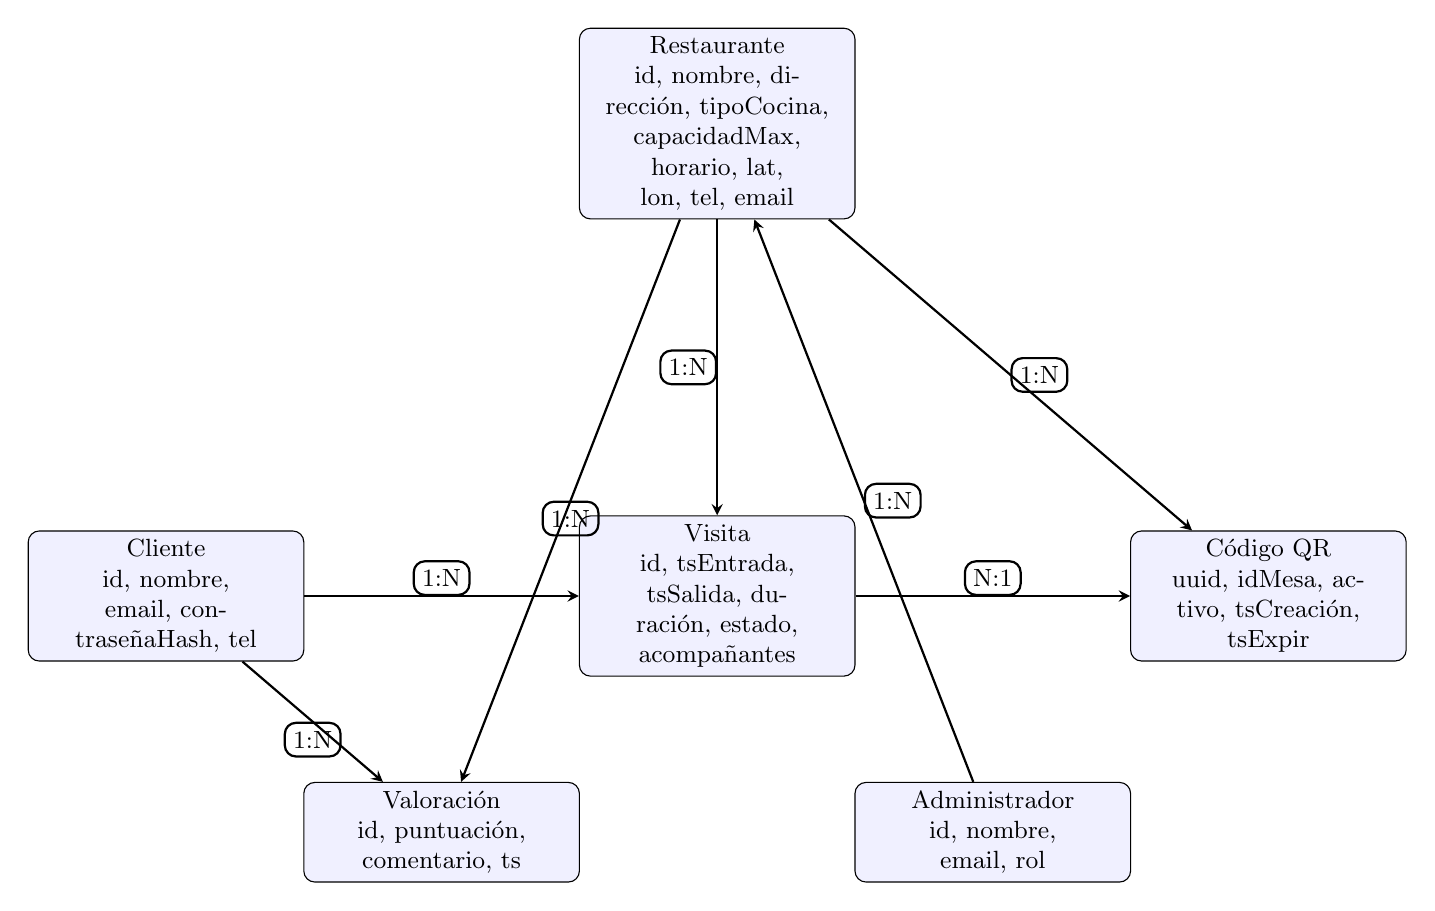
\begin{tikzpicture}[
        every node/.style={draw, rounded corners=4pt, align=center, font=\small, inner sep=3pt},
        class/.style={fill=blue!6, minimum width=3.5cm, minimum height=1.2cm},
        flecha/.style={->, >=stealth, thick}
    ]
    \node[class, text width=3cm] (R) at (0,5) {Restaurante\\\small id, nombre, dirección, tipoCocina, capacidadMax, horario, lat, lon, tel, email};
    \node[class, text width=2.5cm] (C) at (-7,-1) {Cliente\\\small id, nombre, email, contraseñaHash, tel};
    \node[class, text width=2.8cm] (V) at (0,-1) {Visita\\\small id, tsEntrada, tsSalida, duración, estado, acompañantes};
    \node[class, text width=2.5cm] (Q) at (7,-1) {Código QR\\\small uuid, idMesa, activo, tsCreación, tsExpir};
    \node[class, text width=2.5cm] (Va) at (-3.5,-4) {Valoración\\\small id, puntuación, comentario, ts};
    \node[class, text width=2.5cm] (Ad) at (3.5,-4) {Administrador\\\small id, nombre, email, rol};

    \draw[flecha] (R) -- (Q) node[midway,right,font=\small]{1:N};
    \draw[flecha] (R) -- (V) node[midway,left,font=\small]{1:N};
    \draw[flecha] (R) -- (Va) node[midway,below,font=\small]{1:N};
    \draw[flecha] (C) -- (V) node[midway,above,font=\small]{1:N};
    \draw[flecha] (C) -- (Va) node[midway,below,font=\small]{1:N};
    \draw[flecha] (V) -- (Q) node[midway,above,font=\small]{N:1};
    \draw[flecha] (Ad) -- (R) node[midway,right,font=\small]{1:N};
    \end{tikzpicture}
    }
    \caption{Diagrama de Clases — Modelo de Contenido del sistema QR Restaurante.}
    \label{fig:modelo_contenido}
\end{figure}

\subsection{Descripción de las entidades}

\subsubsection{Clase: Restaurante}
Representa al establecimiento registrado en el sistema. Contiene toda la información necesaria para su identificación, geolocalización y operación.

\begin{itemize}
    \item \textbf{Atributos:} id, nombre, dirección, tipoCocina, capacidadMaxima, horarioApertura, horarioCierre, latitud, longitud, teléfono, email, contraseñaHash
    \item \textbf{Relaciones:} 1→N con CódigoQR, 1→N con Visita, 1→N con Valoración
\end{itemize}

\subsubsection{Clase: Cliente}
Representa al usuario final que interactúa con el sistema como comensal.

\begin{itemize}
    \item \textbf{Atributos:} id, nombre, email, contraseñaHash, teléfono
    \item \textbf{Relaciones:} 1→N con Visita, 1→N con Valoración
\end{itemize}

\subsubsection{Clase: Visita}
Registra cada evento de entrada y salida de un cliente en un restaurante. Es la entidad transaccional central del sistema.

\begin{itemize}
    \item \textbf{Atributos:} id, timestampEntrada, timestampSalida (nullable), duraciónMinutos (calculado), estado (activa/completada/cancelada), acompañantes
    \item \textbf{Relaciones:} N→1 con Restaurante, N→1 con Cliente, N→1 con CódigoQR
\end{itemize}

\subsubsection{Clase: CódigoQR}
Almacena los códigos QR generados por cada restaurante y su estado de validez.

\begin{itemize}
    \item \textbf{Atributos:} uuid, idMesa, activo (booleano), fechaCreación, fechaExpiración (nullable)
    \item \textbf{Relaciones:} N→1 con Restaurante, 1→N con Visita
\end{itemize}

\subsubsection{Clase: Valoración}
Registra la puntuación y comentarios que un cliente deja tras su visita.

\begin{itemize}
    \item \textbf{Atributos:} id, puntuación (1-5), comentario (nullable, máx. 500 car.), timestamp
    \item \textbf{Relaciones:} N→1 con Restaurante, N→1 con Cliente
\end{itemize}

\subsubsection{Clase: Administrador}
Usuario del sistema con privilegios elevados para la gestión global.

\begin{itemize}
    \item \textbf{Atributos:} id, nombre, email, contraseñaHash, rol
    \item \textbf{Relaciones:} 1→N con Restaurante (gestión)
\end{itemize}

\subsection{Cardinalidades clave}

\begin{table}[H]
    \centering
    \caption{Resumen de cardinalidades del Modelo de Contenido}
    \label{tab:cardinalidades}
    \begin{tabular}{|c|c|c|c|}
        \hline
        \textbf{Relación} & \textbf{Entidad A} & \textbf{Entidad B} & \textbf{Card.} \\
        \hline
        Registra & Restaurante & CódigoQR & 1:N \\
        \hline
        Registra & Restaurante & Visita & 1:N \\
        \hline
        Recibe & Restaurante & Valoración & 1:N \\
        \hline
        Realiza & Cliente & Visita & 1:N \\
        \hline
        Escribe & Cliente & Valoración & 1:N \\
        \hline
        Utiliza & Visita & CódigoQR & N:1 \\
        \hline
        Gestiona & Administrador & Restaurante & 1:N \\
        \hline
    \end{tabular}
\end{table}

\subsection{Trazabilidad a requisitos}

El Modelo de Contenido se deriva directamente de los requisitos de información definidos en la Práctica 2:

\begin{itemize}
    \item \textbf{RI-01} (Datos del restaurante) → Entidad Restaurante con atributos de identificación, ubicación y configuración.
    \item \textbf{RI-02} (Registro de afluencia) → Entidades Visita y CódigoQR que permiten almacenar el historial de entradas/salidas con timestamps.
    \item \textbf{RF-01} (Registro de establecimientos) → Entidad Restaurante + Administrador.
    \item \textbf{RF-02} (Generación de QR) → Entidad CódigoQR.
    \item \textbf{RF-03} (Registro de entrada por QR) → Entidad Visita vinculada a CódigoQR.
    \item \textbf{RF-04} (Control de aforo) → Atributo capacidadMaxima de Restaurante comparado con el conteo de visitas activas.
\end{itemize}

\section{Modelo de Navegación}

\subsection{Objetivo}
El Modelo de Navegación define la estructura de páginas del sistema y los flujos de navegación entre ellas. Responde a la pregunta: ¿Por qué páginas se desplaza el usuario y cómo se conectan entre sí?

\subsection{Mapa del Sitio}

\begin{figure}[H]
    \centering
    \resizebox{\textwidth}{!}{%
    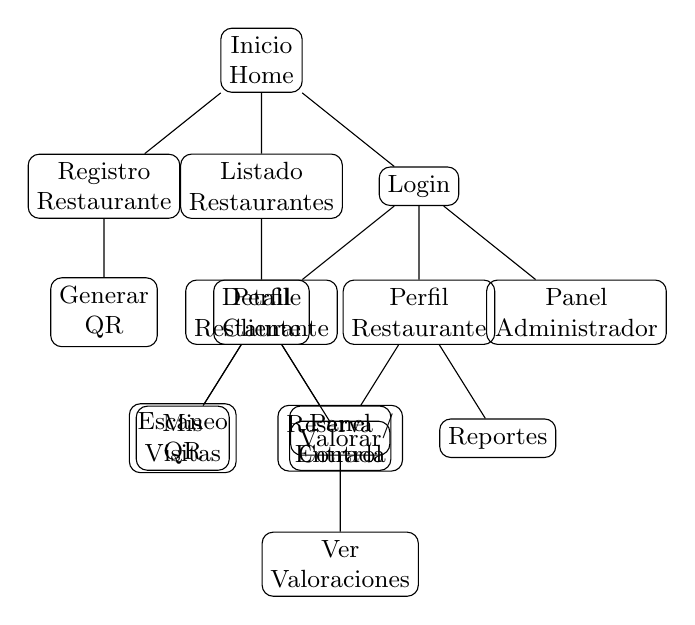
\begin{tikzpicture}[
        every node/.style={draw, rounded corners, align=center, font=\small, inner sep=3pt},
        level distance=1.6cm,
        sibling distance=2cm
    ]
    \node (home) {Inicio\\Home}
        child {node (reg) {Registro\\Restaurante}
            child {node (genqr) {Generar\\QR}}
        }
        child {node (list) {Listado\\Restaurantes}
            child {node (det) {Detalle\\Restaurante}
                child {node (esc) {Escaneo\\QR}}
                child {node (res) {Reserva /\\Entrada}}
            }
        }
        child {node (login) {Login}
            child {node (cli) {Perfil\\Cliente}
                child {node (misvis) {Mis\\Visitas}}
                child {node (val) {Valorar}
                    child {node (vdet) {Ver\\Valoraciones}}
                }
            }
            child {node (rest) {Perfil\\Restaurante}
                child {node (panel) {Panel\\Control}}
                child {node (report) {Reportes}}
            }
            child {node (admin) {Panel\\Administrador}}
        };
    \end{tikzpicture}
    }
    \caption{Mapa del Sitio — Estructura de navegación del sistema.}
    \label{fig:mapa_sitio}
\end{figure}

\subsection{Diagramas de Navegación por Actor}

\subsubsection{Cliente (Visitante / Usuario Registrado)}

\begin{figure}[H]
    \centering
    \resizebox{0.85\textwidth}{!}{%
    \begin{tikzpicture}[
        every node/.style={draw, rounded corners, align=center, minimum width=1.8cm, font=\small, inner sep=2pt},
        flecha/.style={->, >=stealth, thick}
    ]
    \node (home) [startstop] {Home};
    \node (list) [process, below of=home, yshift=-0.8cm] {Listado};
    \node (filtro) [process, right of=list, xshift=2.5cm] {Filtros};
    \node (det) [process, below of=list, yshift=-0.8cm] {Detalle};
    \node (scan) [process, left of=det, xshift=-2.5cm] {Escaneo\\QR};
    \node (entrada) [process, below of=det, yshift=-0.8cm] {Entrada};
    \node (misvisitas) [process, right of=det, xshift=2.5cm] {Mis\\Visitas};
    \node (salida) [process, below of=misvisitas, yshift=-0.8cm] {Salida};
    \node (valorar) [process, right of=misvisitas, xshift=2.5cm] {Valorar};

    \draw [flecha] (home) -- (list);
    \draw [flecha] (list) -- (det);
    \draw [flecha] (list) -- (filtro);
    \draw [flecha] (filtro) |- (list);
    \draw [flecha] (det) -- node[left, font=\small] {Escaneo} (scan);
    \draw [flecha] (det) -- node[right, font=\small] {Entrar} (entrada);
    \draw [flecha] (det) -- (misvisitas);
    \draw [flecha] (misvisitas) -- (salida);
    \draw [flecha] (salida) -- node[above, font=\small] {Valorar?} (valorar);
    \draw [flecha] (scan.south) |- (entrada);
    \end{tikzpicture}
    }
    \caption{Diagrama de Navegación — Actor: Cliente.}
    \label{fig:nav_cliente}
\end{figure}

\subsubsection{Restaurante (Propietario / Gerente)}

\begin{figure}[H]
    \centering
    \resizebox{0.65\textwidth}{!}{%
    \begin{tikzpicture}[
        every node/.style={draw, rounded corners, align=center, minimum width=2cm, font=\small, inner sep=2pt},
        flecha/.style={->, >=stealth, thick}
    ]
    \node (login) [startstop] {Login};
    \node (panel) [process, below of=login, yshift=-0.8cm] {Panel\\Control};
    \node (aqr) [process, left of=panel, xshift=-2.5cm] {Gestión\\QR};
    \node (genqr) [process, below of=aqr, yshift=-0.8cm] {Generar\\QR};
    \node (reportes) [process, right of=panel, xshift=2.5cm] {Reportes};
    \node (afluencia) [process, below of=reportes, yshift=-0.8cm] {Afluencia};
    \node (datos) [process, below of=panel, yshift=-0.8cm] {Mis\\Datos};

    \draw [flecha] (login) -- (panel);
    \draw [flecha] (panel) -- (aqr);
    \draw [flecha] (panel) -- (reportes);
    \draw [flecha] (panel) -- (datos);
    \draw [flecha] (aqr) -- (genqr);
    \draw [flecha] (reportes) -- (afluencia);
    \end{tikzpicture}
    }
    \caption{Diagrama de Navegación — Actor: Restaurante.}
    \label{fig:nav_restaurante}
\end{figure}

\subsubsection{Administrador}

\begin{figure}[H]
    \centering
    \resizebox{0.55\textwidth}{!}{%
    \begin{tikzpicture}[
        every node/.style={draw, rounded corners, align=center, minimum width=2cm, font=\small, inner sep=2pt},
        flecha/.style={->, >=stealth, thick}
    ]
    \node (login) [startstop] {Login Admin};
    \node (gestion) [process, below of=login, yshift=-0.8cm] {Gestión\\Restaurantes};
    \node (reportes) [process, right of=gestion, xshift=2.5cm] {Reportes\\Globales};
    \node (usuarios) [process, below of=gestion, yshift=-0.8cm] {Gestión\\Usuarios};
    \node (config) [process, below of=usuarios, yshift=-0.8cm] {Configuración\\Sistema};

    \draw [flecha] (login) -- (gestion);
    \draw [flecha] (gestion) -- (reportes);
    \draw [flecha] (gestion) -- (usuarios);
    \draw [flecha] (usuarios) -- (config);
    \end{tikzpicture}
    }
    \caption{Diagrama de Navegación — Actor: Administrador.}
    \label{fig:nav_admin}
\end{figure}

\section{Modelo de Proceso}

\subsection{Objetivo}
El Modelo de Proceso define la lógica de negocio que ocurre por detrás de cada acción del usuario. Se compone de dos niveles:

\begin{enumerate}
    \item \textbf{Estructura de Proceso:} las clases de proceso (actividades agrupadas funcionalmente).
    \item \textbf{Flujo de Proceso:} los diagramas de actividad detallados (ya desarrollados en la Práctica 2).
\end{enumerate}

\subsection{Estructura de Proceso}

\begin{figure}[H]
    \centering
    \resizebox{\textwidth}{!}{%
    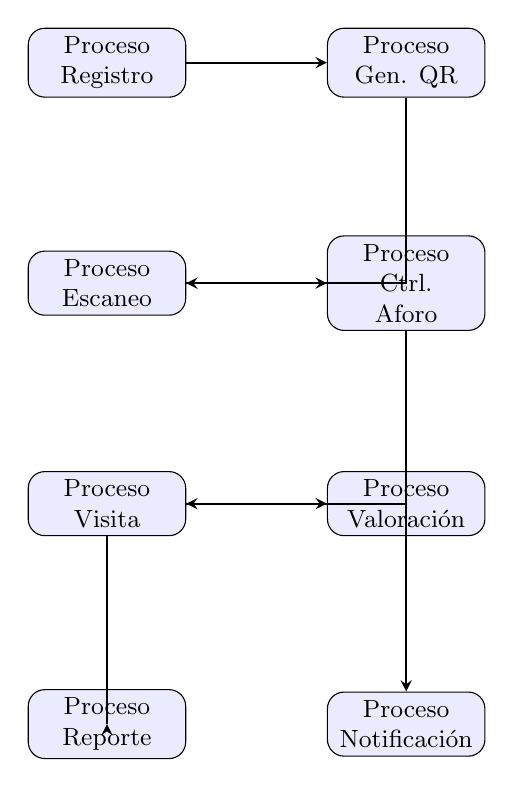
\begin{tikzpicture}[
        every node/.style={draw, rounded corners=6pt, align=center, font=\small, inner sep=3pt},
        proc/.style={fill=blue!8, minimum width=2cm, minimum height=0.8cm},
        flecha/.style={->, >=stealth, thick}
    ]
    \node (p1) [proc] {Proceso\\Registro};
    \node (p2) [proc, right of=p1, xshift=2.8cm] {Proceso\\Gen. QR};
    \node (p3) [proc, below of=p1, yshift=-1.8cm] {Proceso\\Escaneo};
    \node (p4) [proc, right of=p3, xshift=2.8cm] {Proceso\\Ctrl.\\Aforo};
    \node (p5) [proc, below of=p3, yshift=-1.8cm] {Proceso\\Visita};
    \node (p6) [proc, right of=p5, xshift=2.8cm] {Proceso\\Valoración};
    \node (p7) [proc, below of=p5, yshift=-1.8cm] {Proceso\\Reporte};
    \node (p8) [proc, right of=p7, xshift=2.8cm] {Proceso\\Notificación};

    \draw [flecha] (p1) -- (p2);
    \draw [flecha] (p2) |- (p3);
    \draw [flecha] (p3) -- (p4);
    \draw [flecha] (p4) |- (p5);
    \draw [flecha] (p5) -- (p6);
    \draw [flecha] (p5) |- (p7);
    \draw [flecha] (p4) -- (p8);
    \end{tikzpicture}
    }
    \caption{Estructura de Proceso — Clases de proceso y sus interrelaciones.}
    \label{fig:estructura_proceso}
\end{figure}

\subsection{Descripción de cada Clase de Proceso}

\begin{table}[H]
    \centering
    \caption{Clases de Proceso y su correspondencia con requisitos}
    \label{tab:clases_proceso}
    \begin{tabularx}{\textwidth}{|l|X|l|}
        \hline
        \textbf{Clase de Proceso} & \textbf{Descripción} & \textbf{Req.} \\
        \hline
        ProcesoRegistro & Alta de restaurante, validación de datos y asignación de UUID & RF-01 \\
        \hline
        ProcesoGeneraciónQR & Creación de código único por mesa/acceso, vinculación a restaurante & RF-02 \\
        \hline
        ProcesoEscaneo & Decodificación de QR, validación de hash y expiración & RF-03 \\
        \hline
        ProcesoControlAforo & Comparación ocupación/capacidad, alertas y modo restrictivo & RF-04, RNF-03 \\
        \hline
        ProcesoVisita & Registro entrada/salida, cálculo de duración y gestión de acompañantes & RF-03, RI-02 \\
        \hline
        ProcesoValoración & Captura de puntuación, validación de contenido y recálculo de media & Implícito \\
        \hline
        ProcesoReporte & Agregación de métricas, generación de estadísticas y exportación & Implícito \\
        \hline
        ProcesoNotificación & Alertas en tiempo real al restaurante (umbrales de aforo) & RNF-03 \\
        \hline
    \end{tabularx}
\end{table}

\subsection{Flujos de Proceso}

Los flujos detallados de cada proceso ya fueron definidos en los 8 diagramas de actividad desarrollados durante la Práctica 2, que se recogen a continuación para referencia cruzada:

\begin{enumerate}
    \item \textbf{Diagrama 1:} Registro de Restaurante (RF-01)
    \item \textbf{Diagrama 2:} Generación de Código QR (RF-02)
    \item \textbf{Diagrama 3:} Escaneo y Registro de Entrada (RF-03)
    \item \textbf{Diagrama 4:} Registro de Salida (RF-03, RI-02)
    \item \textbf{Diagrama 5:} Visualización de Restaurantes Disponibles (RF-03)
    \item \textbf{Diagrama 6:} Control de Aforo en Tiempo Real (RF-04)
    \item \textbf{Diagrama 7:} Valoración de Restaurante (Req. implícito)
    \item \textbf{Diagrama 8:} Reporte de Afluencia — Administrador (Req. implícito)
\end{enumerate}

Los diagramas con su lógica completa se adjuntan en formato Mermaid en el anexo complementario incluido en el repositorio del proyecto.

\section{Modelo de Presentación}

\subsection{Objetivo}
El Modelo de Presentación define la apariencia y comportamiento de cada interfaz del sistema. Describe cómo el usuario percibe e interactúa con las funcionalidades descritas en los modelos anteriores.

\subsection{Metodología}
En lugar de wireframes estáticos (que requieren herramientas como Figma o Balsamiq), se opta por tablas de especificación de vistas, estándar aceptado en proyectos UWE académicos. Este formato es más trazable y permite al profesor verificar la cobertura de requisitos de forma directa.

\subsection{Vistas del Sistema}

A continuación se define cada vista del sistema con sus componentes, actores asociados y requisitos cubiertos.

\subsubsection{Vista 1: Home / Inicio}
\begin{itemize}
    \item \textbf{Componentes:} Cabecera (logo, menú login/registro), Hero Section (eslogan, CTA de búsqueda), Sección de destacados (top 5 restaurantes), Filtros rápidos, Footer
    \item \textbf{Actor:} Cliente (anon/autenticado), Restaurante, Admin
    \item \textbf{Requisitos:} RF-03, RF-04
\end{itemize}

\subsubsection{Vista 02: Listado de Restaurantes}
\begin{itemize}
    \item \textbf{Componentes:} Barra de filtros (tipo comida, zona/radio), ordenación (distancia/valoración/disponibilidad), Grid de cards (foto, nombre, tipo, distancia, valoración, plazas libres, botón detalles), paginación, mapa opcional
    \item \textbf{Actor:} Cliente
    \item \textbf{Requisitos:} RF-03, RNF-01
\end{itemize}

\subsubsection{Vista 03: Detalle de Restaurante}
\begin{itemize}
    \item \textbf{Componentes:} Cabecera (foto, nombre, tipo, valoración media), Información (dirección, horario, capacidad ocupación/máxima, distancia), Código QR, Botón ``Escanear para entrar'', Sección de valoraciones
    \item \textbf{Actor:} Cliente, Restaurante
    \item \textbf{Requisitos:} RF-02, RF-03, RNF-01
\end{itemize}

\subsubsection{Vista 04: Escaneo QR / Registro de Entrada}
\begin{itemize}
    \item \textbf{Componentes:} Visor de cámara con recuadro de escaneo, resultado del escaneo (nombre, dirección, capacidad), validación de QR (expirado/inválido/lleno), formulario de acompañantes (0-10), botón confirmar entrada
    \item \textbf{Actor:} Cliente
    \item \textbf{Requisitos:} RF-03, RF-04, RNF-02
\end{itemize}

\subsubsection{Vista 05: Registro de Restaurante (Admin/Propietario)}
\begin{itemize}
    \item \textbf{Componentes:} Formulario completo (nombre, dirección con geocodificación, tipo cocina, capacidad máxima, horario, tel, email), validación en tiempo real, mapa de ubicación, botón registrar, confirmación con resumen y QR descargable
    \item \textbf{Actor:} Administrador, Restaurante
    \item \textbf{Requisitos:} RF-01, RF-02
\end{itemize}

\subsubsection{Vista 06: Panel de Control del Restaurante}
\begin{itemize}
    \item \textbf{Componentes:} Dashboard con gráfico de ocupación en tiempo real (verde/amarillo/rojo), KPIs (aforo actual/máximo, visitas hoy, duración media, acompañantes media), gestión de QR (lista con UUID, mesa, estado, botón generar), alertas automáticas de aforo, sección histórica
    \item \textbf{Actor:} Restaurante
    \item \textbf{Requisitos:} RF-04, RI-02, RNF-03
\end{itemize}

\subsubsection{Vista 07: Mis Visitas (Cliente)}
\begin{itemize}
    \item \textbf{Componentes:} Lista de visitas (restaurante, fecha/hora, estado, duración), botón registrar salida con confirmación de acompañantes, botón valorar tras salida
    \item \textbf{Actor:} Cliente
    \item \textbf{Requisitos:} RF-03, RI-02
\end{itemize}

\subsubsection{Vista 08: Valoración de Restaurante}
\begin{itemize}
    \item \textbf{Componentes:} Selector de estrellas (1-5), campo de comentario (máx. 500 caracteres con contador), validación de contenido ofensivo, botón enviar
    \item \textbf{Actor:} Cliente
    \item \textbf{Requisitos:} Requisito implícito
\end{itemize}

\subsubsection{Vista 09: Reportes (Administrador)}
\begin{itemize}
    \item \textbf{Componentes:} Selector de tipo de reporte (restaurante/fecha/horario/comparativo), selector de período, panel de métricas (entradas, salidas, duración media, peak hours), gráficos (barras, línea, circular), exportación PDF/Excel/CSV
    \item \textbf{Actor:} Administrador
    \item \textbf{Requisitos:} RI-02, requisito implícito (reportes)
\end{itemize}

\subsection{Correspondencia Vistas $\leftrightarrow$ Requisitos}

\begin{table}[H]
    \centering
    \caption{Matriz de trazabilidad: Vistas $\times$ Requisitos}
    \label{tab:trazabilidad}
    \small
    \begin{tabular}{|c|c|c|c|c|c|c|c|}
        \hline
        \textbf{Vista} & \textbf{RF-01} & \textbf{RF-02} & \textbf{RF-03} & \textbf{RF-04} & \textbf{RI-01} & \textbf{RI-02} & \textbf{RNF} \\
        \hline
        V-01 Home      & --- & contrib. & contrib. & ---  & --- & --- & ✓ \\ \hline
        V-02 Listado   & --- & contrib. & contrib. & ---  & --- & --- & ✓ \\ \hline
        V-03 Detalle   & --- & contrib. & contrib. & contrib. & contrib. & --- & ✓ \\ \hline
        V-04 Escaneo   & --- & contrib. & contrib. & contrib. & --- & --- & ✓ \\ \hline
        V-05 Registro  & contrib. & contrib. & --- & ---  & contrib. & --- & ✓ \\ \hline
        V-06 Panel     & --- & contrib. & --- & contrib. & --- & contrib. & contrib. \\ \hline
        V-07 Mis Vis.  & --- & --- & contrib. & ---  & --- & contrib. & ✓ \\ \hline
        V-08 Valorar   & --- & --- & contrib. & ---  & --- & --- & ✓ \\ \hline
        V-09 Reportes  & --- & --- & --- & ---  & --- & contrib. & contrib. \\ \hline
    \end{tabular}

    \vspace{0.3cm}
    contrib. = contribución indirecta; ✓ = satisface directamente; RNF = RNF-01/02/03.
\end{table}

\subsection{Diagrama de Secuencia del Flujo Principal}

A continuación se presenta el diagrama de secuencia del flujo más crítico del sistema: el escaneo de QR y registro de entrada.

\begin{figure}[H]
    \centering
    \resizebox{0.85\textwidth}{!}{%
    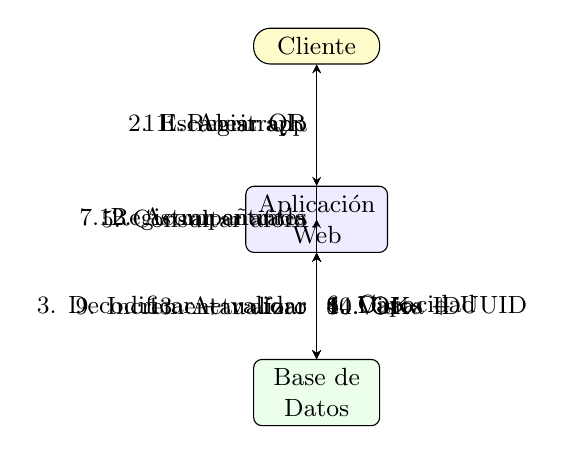
\begin{tikzpicture}[
        actor/.style={draw, rounded corners=6pt, fill=yellow!20, minimum width=1.6cm, align=center, font=\small},
        box/.style={draw, rounded corners=3pt, fill=blue!7, minimum width=1.8cm, align=center, font=\small},
        dbase/.style={draw, rounded corners=3pt, fill=green!8, minimum width=1.6cm, align=center, font=\small},
        flecha/.style={->, >=stealth}
    ]
    \node (cliente) [actor] {Cliente};
    \node (app) [box, below of=cliente, yshift=-1.2cm] {Aplicación\\Web};
    \node (db) [dbase, below of=app, yshift=-1.2cm] {Base de\\Datos};

    \draw [flecha] (cliente) -- node[left, font=\small] {1. Abrir app} (app);
    \draw [flecha] (cliente) -- node[left, font=\small] {2. Escanear QR} (app);
    \draw [flecha] (app) -- node[left, font=\small] {3. Decodificar + validar} (db);
    \draw [flecha] (db) -- node[right, font=\small] {4. Datos + UUID} (app);
    \draw [flecha] (app) -| node[left, font=\small] {5. Consultar aforo} (db);
    \draw [flecha] (db) -- node[right, font=\small] {6. Capacidad} (app);
    \draw [flecha] (app) -| node[left, font=\small] {7. Registrar entrada} (db);
    \draw [flecha] (db) -- node[right, font=\small] {8. Visita ID} (app);
    \draw [flecha] (app) -- node[left, font=\small] {9. Incrementar aforo} (db);
    \draw [flecha] (db) -- node[right, font=\small] {10. OK} (app);
    \draw [flecha] (app) -- node[left, font=\small] {11. Registrado} (cliente);
    \draw [flecha] (cliente) |- node[left, pos=0.6, font=\small] {12. Acompañantes} (app);
    \draw [flecha] (app) -- node[left, font=\small] {13. Actualizar} (db);
    \draw [flecha] (db) -- node[right, font=\small] {14. OK} (app);
    \draw [flecha] (app) -- (cliente);
    \end{tikzpicture}
    }
    \caption{Diagrama de Secuencia — Escaneo QR y Registro de Entrada.}
    \label{fig:secuencia_entrada}
\end{figure}

\section{Decisiones de Diseño}

\begin{enumerate}
    \item \textbf{Modelo relacional sobre NoSQL:} Se opta por una base de datos relacional (por ejemplo, PostgreSQL) por la naturaleza transaccional del sistema (entradas/salidas con consistencia de aforo), donde la integridad referencial es crítica.
    \item \textbf{Trazabilidad de requisitos:} Cada modelo presenta una sección explícita de trazabilidad que conecta los requisitos de la Práctica 2 con los artefactos de diseño generados.
    \item \textbf{Separación de actores:} Se mantiene una distinción clara entre los tres roles (cliente, restaurante, administrador) tanto en la navegación como en la presentación, siguiendo el principio de \textit{least privilege}.
    \item \textbf{Diseño responsive:} Los requisitos no funcionales (RNF-01) exigen que todas las vistas sean adaptables a dispositivos móviles, dado que el flujo principal (escaneo de QR) se ejecuta desde un teléfono.
    \item \textbf{Modelo de Proceso como orquestador:} Los procesos de negocio (registro, escaneo, valoración) se modelan como clases de proceso independientes, lo que facilita su implementación futura como servicios o microservicios.
\end{enumerate}

\section{Resumen}

En esta práctica se han definido los cuatro modelos arquitectónicos exigidos por la metodología UWE:

\begin{itemize}
    \item \textbf{Modelo de Contenido:} 6 entidades con sus relaciones y cardinalidades, trazables a los requisitos RI y RF definidos en la Práctica 2.
    \item \textbf{Modelo de Navegación:} Mapa del sitio y diagramas de navegación por cada actor del sistema (cliente, restaurante, administrador).
    \item \textbf{Modelo de Proceso:} 8 clases de proceso documentadas, con su correspondencia a requisitos y referencia a los 8 diagramas de actividad ya generados.
    \item \textbf{Modelo de Presentación:} 9 vistas especificadas mediante tablas de componentes, con matriz de trazabilidad a requisitos.
\end{itemize}

Estos artefactos constituyen la base sobre la que se construirá la implementación y las pruebas descritas en la Práctica 4.